\documentclass{ximera}

\title{Disks and Washers: Practice}
\author{Pat Smith}

\begin{document}
\begin{abstract}
  A regression test of \texttt{answer}.
\end{abstract}
\maketitle

\begin{problem}
\begin{image}
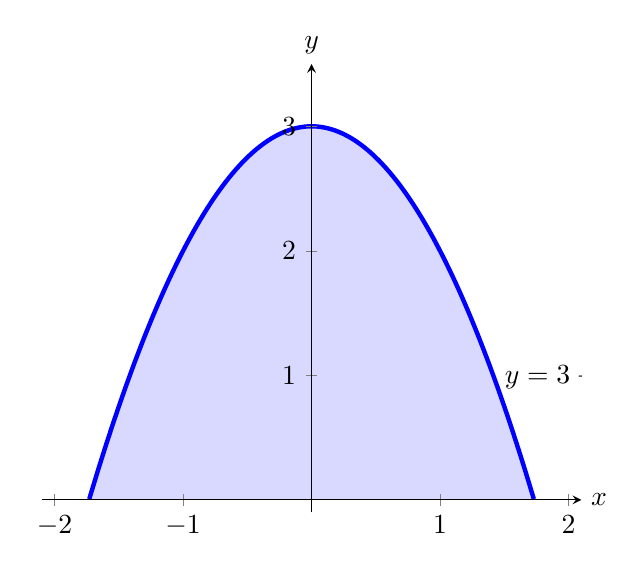
\begin{tikzpicture}
\begin{axis}[axis y line=middle,axis x line=middle,name=myplot,axis on top,ymin=-.1,ymax=3.5,xmin=-2.1,xmax=2.1]
\addplot [ {blue!15!white},fill={blue!15!white}, samples=50,domain=-1.73:1.73] {3-x^2};
\addplot [smooth,ultra thick, {blue}, samples=50,domain=-1.73:1.73] {3-x^2};
\addplot [black] (2,1) node  {\(y=3-x^2\)};
\end{axis}
\node [right] at (myplot.right of origin) {\(x\)};
\node [above] at (myplot.above origin) {\(y\)};
\end{tikzpicture}
\end{image}
A region of the cartesian plane is shaded. use the disk/washer method to find the volume of the solid of revolution formed by revolving the region about the \(x\)-axis.
\begin{prompt}
\[ V = \answer{\frac{48\pi\sqrt{3}}{5}} \]
\end{prompt}



\end{problem}


\end{document}
